%%%%
\documentclass[a4paper,11pt]{article}
%%%%
%%%%
%PACKAGES______________________________________________________________________________________
\usepackage{simplewick} %Allows Wick Notation
\usepackage{slashed} %Allows feynman slash notation 
\usepackage{graphicx} % graphics, pictures, figures
\usepackage{caption}
\usepackage{subcaption}
\usepackage{verbatim} % importing numerical scripts
\usepackage{multicol, float} % placing floats in right places
\usepackage{algpseudocode} % no idea...
\usepackage[utf8]{inputenc}
\usepackage{amssymb} %needed if not using mathdesign
\usepackage{amsmath}
\usepackage[OT1]{fontenc}
\usepackage{lmodern} %gfsartemisia, times, boisik, et cetera
\usepackage{braket} %dirac notation
\usepackage[cm]{fullpage} % for fulpage style
\usepackage{bm} % boldface vectors
\usepackage{float} % placing floats
\usepackage{relsize} % for \mathlarger command
\usepackage{mathrsfs} %?
\usepackage{textgreek} % cb-greek class
\usepackage{sectsty} % for centering sections
\usepackage{textcomp } % for nr. symbol
\usepackage[usenames, dvipsnames]{color} % defining own colors
\usepackage{type1cm} % scalable fonts
\usepackage{lettrine} % larger first letter in paragraph.
\usepackage{listings} % code-snippets in the text
\usepackage{background} % used for top page text
%\usepackage{niceframe} % for old-school double frame
\usepackage{tikz} % figure config/ creation
%\usepackage{bbold}
%\usepackage{swrule} % for fancy line
%\usepackage{pdfpages} % for importing pdf

%%%%
%%%% SET-UP NEEDED FOR FURTHER PACKAGES
%%%%
\definecolor{hyperclrblue}{RGB}{30,90,125} %Definind own color ; blue
\definecolor{hyperclrorng}{RGB}{210,100,45}%Definind own color
\definecolor{hyperclrgreen}{RGB}{60,120,20}%Definind own color
\usepackage[colorlinks = true,
linkcolor = hyperclrblue,
urlcolor = blue,
citecolor = blue,
anchorcolor = blue]{hyperref} % link package
\usepackage{pgfplots} % to plot directly into latex
\pgfplotsset{compat=1.5} % needed forpgfplots
\usepackage{framed, color} % for framing/shaded box
\definecolor{shadecolor}{cmyk}{0,0,0.185,0} % color for shaded box
\usepackage{fancybox}
\usepackage[sc]{titlesec} % title package
%_______________________________________________________________________________________________
%NEW COMMANDS_________________________________________________________________________________
%\renewcommand*{\thefootnote}{$\dagger$} % creating dagger footnote
\newcommand*{\boisik}{\fontfamily{bsk}\selectfont} % change font to boisik command
\newcommand{\wf}{\text{\textpsi}} % defining wavefunctions as cbgreek class.
\newcommand{\bwf}{\text{\textPsi}} % defining Wavefunctions as cbgreek class.
\newcommand{\Q}{\hat{\text{\boisik Q}}} % defining operator-style 'Q'
\newcommand{\nlm}{\ket{n\ell m_\ell}} % defining wavefunctions as cbgreek class.
\newcommand{\nlmz}{\ket{n\ell m_\ell;0}} % defining wavefunctions as cbgreek class.
\newcommand{\nlmt}{\ket{n\ell m_\ell;t}} % defining wavefunctions as cbgreek class.
%_____________________________________________
%\numberwithin{equation}{section} %equations labeled by section
\sectionfont{\centering} % centering sections with 'sectsty'
\subsectionfont{\centering} % centering sections with 'sectsty'
\definecolor{myclr}{RGB}{190,90,20} %Definind own color
\renewcommand{\thesection}{\Roman{section}.} % Roman numerals for sections
\renewcommand{\thesubsection}{\Alph{subsection}} % Roman numerals for subsections
\titleformat{\section}{\large\scshape\centering}{\thesection}{1em}{} % Change the look of the section titles
\titleformat{\subsection}{\normalsize\centering\bfseries}{\thesubsection.}{1em}{} % Change the look of the section titles
\setlength{\columnsep}{0.7cm}
%______________________________________________________________________________________________
%%%%
%%%%_________________________________________________________________________________________
\begin{document}
%%%% TOP PAGE TEXT
{\SetBgContents{ \textit{{\small\textsc{ Ask J. Markestad, Thorbjørn V. Larsen Universitetet i Oslo. \hspace{3.5cm} \textit{\today}}}}}
\SetBgScale{1}
\SetBgColor{black}
\SetBgAngle{0}
\SetBgOpacity{1}
\SetBgPosition{current page.north east}
\SetBgVshift{-1.2cm}
\SetBgHshift{-10.5cm}
%%%% CREATING TITLE HEADER
$$\:$$
\begin{center}
	\vspace{0.2cm}%\boisik
	\fontsize{15}{15}\selectfont \textsc{ 3D Quantum Mechanical oscillator with interaction term solved with Jacobi's method}\\
	%{in}}\\
	\fontsize{13}{13}\selectfont \textsc{Fys $\textnormal{{4150}}$: Project 2}\\
	\vspace{0.4cm}
	\fontsize{12}{12}\selectfont {\textsc{ Ask J. Markestad, Thorbjoern V. Larsen }}\\
	\vspace{0.5cm}
\end{center}
%%%%
%%%%
%______________________________________________________________________________________________
%%%%
%%%%
	
%\includegraphics[scale = 0.48]{line}
\rule{\textwidth}{0.3pt}\par
		
%---------------------------------------------------------------------------------------------------------------------------------------
\begin{abstract}
	We rewrite Schrödinger equation for harmonics oscillator potential for electron two particle wave-functions with and without Coulomb interaction into a unit-less equation. We then solve this equation by linearizing it, and using Jacobi's method of similarity transformations \cite{M.Hjort-Jensen_CompFys} to find both eigenvalues and eigenfunctions, meanwhile trying to optimize the calculation with respect to the approximation for the boundary condition versus the number of iteration points. We then compare the calculation speed with a faster method implemented in an eigenvalue equation solver from the armadillo library\cite{Armadillo}.
\end{abstract}



		
\section*{Introduction}

Eigenvalue equations are the heart and soul of quantum mechanics, where the fundamental equation is the Schrödinger equation. Having a firm grasp on how to solve eigenvalue equations numerically and the difficulties that it entails are important tools in any physicists arsenal. In this article we will show how to rewrite the Schrödinger equation into a dimensionless form and how to solve it, in the process creating a eigenvalue solver. To illustrate this we will use a physically interesting example; two electrons trapped in a harmonic oscillator potential. This allows us to showcase some of the problems of linearizing and discretizing the Schrödinger equations with respect to the boundary conditions and their physical relevance. We will then use a general solver based on Jacobi's method of similarity transformations in a brute force way to illustrate how these problems affect the accuracy of the solution as well illustrate the ideas behind solving eigenvalue equations, as well as using the results to tell us about how the forces involved interact for different oscillator frequencies. We will finally use a smarter eigenvalue solver from the Armadillo library \cite{Armadillo} to showcase the speed inefficiency of Jacobi's method.
		
		
		
		
\section*{Theory and Algorithms}

Generally we can split up the Schrödinger equation into a radial equation and spherical equation, for a spherically symmetric potential. The spherical equation will be potential independent such that we can solve it once and for all for any situation where this symmetry is observed, and are thus not necessary to calculate. We will thus only concern ourselves with the radial equation, and we will further confine ourselves to systems with zero angular momentum (including it would only constitute an extra term in the potential and can be trivially added if one is interested). As stated in the introduction we will consider a two electron system with a harmonic oscillator potential, and we thus have the equation:

\begin{equation}
\left(- \frac{\hbar^2}{2m}\frac{d^2}{d r_1^2} - \frac{\hbar^2}{2m}\frac{d^2}{d r_2^2} + \frac{1}{2}k r_1^2 + \frac{1}{2}k r_2^2 + \frac{\beta e^2}{|\mathbf{r}_1 - \mathbf{r}_2|}\right) \: u(r_1,r_2) = E_{tot} \: u(r_1,r_2)
\label{schro_radial}
\end{equation} 

Where m is the mass of one electron, $k = m \omega^2 $, and $ \beta e^2 = 1.44 eVnm$. We will then introduce a change of coordinates into center om mass radius, $ R = \frac{1}{2} (r_1 + r_2) $, and relative distance, $ r = r_1 - r_2 $, and rewrite eq.\ref{schro_radial} n terms of these coordinates:

\begin{equation}
\left(- \frac{\hbar^2}{m}\frac{d^2}{d r^2} - \frac{\hbar^2}{4m}\frac{d^2}{d R^2} + \frac{1}{4}k r^2 + k R^2 + \frac{\beta e^2}{r}\right) \: u(r,R) = E_{tot} \: u(r,R)
\label{schro_radial_CM_rel}
\end{equation}

We can then use separation of variables to get one equation for the relative distance and one for the center of mass radius. However, the center of mass equation is the standard harmonic oscillator equation which has a known solution, and can in any case be solved by setting the coulomb interaction to zero in the relative distance equation. We will therefore focus on the relative distance equation moving forward. 

\begin{equation}
\left(- \frac{\hbar^2}{m}\frac{d^2}{d r^2} + \frac{1}{4}k r^2+ \frac{\beta e^2}{r}\right) \: \psi(r) = E_{r} \: \psi(r)
\label{schro_radial_rel}
\end{equation}

We will now introduce the dimensionless variable $\rho = r/\alpha$ and divide throughout by $\frac{\hbar^2}{m} $ to get:

\begin{equation}
\left(- \frac{d^2}{d \rho^2} + \frac{1}{4}\frac{m k}{\hbar^2} \alpha^4  \rho^2+ \frac{m \alpha \beta e^2}{\rho \hbar^2}\right) \: \psi(r) = \frac{m \alpha^2}{\hbar^2}E_{r} \: \psi(r)
\label{dimless_schro_radial_rel}
\end{equation}

Since we want to analyze the system for different oscillator frequencies we will define a new dimensionless frequency $\omega_r^2 = \frac{1}{4}\frac{m k}{\hbar^2} \alpha^4 $ and choose $\alpha$ such that the factor $\frac{m \alpha \beta e^2}{ \hbar^2} = 1$. Further defining $\lambda = \frac{m \alpha^2}{\hbar^2}E_{r} $ we get the equation:

\begin{equation}
\left(- \frac{d^2}{d \rho^2} + \omega_r^2  \rho^2+ \frac{1}{\rho}\right) \: \psi(r) = \lambda \: \psi(r)
\label{dimless_schro_radial_rel_simple}
\end{equation}

We will proceed with the discretization and militarization of the derivative and the equation as in ref\cite{Project1}. This will give us the matrix equation:


\begin{equation}
\begin{pmatrix}
	\frac{2}{h^2} + \omega_r^2 \rho_1 + \frac{1}{\rho_1} & \frac{-1}{h^2} & 0 & ... & ... & 0 \\
	\frac{-1}{h^2} & \frac{2}{h^2} + \omega_r^2 \rho_2 + \frac{1}{\rho_2} & \frac{-1}{h^2} & 0 & ... & 0 \\
	... & ... & ... & ... & ... & ... \\
	0 & ... & 0 & \frac{-1}{h^2} & \frac{2}{h^2} + \omega_r^2 \rho_{n-2} + \frac{1}{\rho_{n-2}} & \frac{-1}{h^2} \\
	0 & 0 & ... & 0 & \frac{-1}{h^2} & \frac{2}{h^2} + \omega_r^2 \rho_{n-1} + \frac{1}{\rho_{n-1}} 
	\end{pmatrix} \begin{pmatrix}
	\psi_1\\
	\psi_2\\
	...\\
	...\\
	\psi_n
	\end{pmatrix} = \lambda \begin{pmatrix}
	\psi_1 \\
	\psi_2  \\
	... \\
	... \\
	\psi_n  \\
	\end{pmatrix}
\end{equation}		

Where we have excluded the endpoints as they are known from the boundary conditions. But as previously hinted, we have to be careful with the implementation of these boundary conditions. In quantum mechanics we relate the absolute squared of the wave-functions to a probability distribution. We therefore require the wave-functions to be normalizable and thus we need the boundary conditions that the wave-function goes to zero as we approach infinity. In the radial system these conditions become $\psi(r=0) = 0, \: \: \: \psi(r=\infty) = 0$, and the same conditions apply for $\rho$ as a variable. However, we cannot actually represent infinity in a computer. Instead we need to set some large value for $\rho_{max}$ instead for a boundary condition. This presents a problem as our step length is defined by $h = \frac{\rho_{max}-\rho_{min}}{n}$, where n is the number of points used in the discretization, so for a large $\rho_{max}$ we need a larger grid size to keep our precision up, which means higher computational time. Therefore what $\rho_{max}$ should be depends on the potential used, if we have a high frequency then the wave functions will be forced narrow and we can get away with a small $\rho_{max}$ and we can get a higher accuracy without much cost to the computation time, while for a small frequency we have the opposite problem. We will therefore choose n based on the frequency used in the calculation and some precision parameter such that everything scales properly. \\

Jacobi's method is based digitalization by means of similarity transformations. Similarity transformations are unitary transformations that preserve several key characteristics of the transformed matrix, namely the eigenvalues, orthogonality and the inner product. The theory is simple, given a transformation $\mathbf{S}$ and a matrix $\mathbf{A}$ such that $\mathbf{S}^{\dagger}\mathbf{S} = 1$ and $\mathbf{S}^{\dagger}\mathbf{A}\mathbf{S} = \mathbf{D}$ where $\mathbf{D}$ is a diagonal matrix then:

\begin{equation}
\mathbf{A} \vec{v} = \lambda \vec{v} \: \: \therefore \: \: \mathbf{S}^{\dagger}\mathbf{A}\mathbf{S}\mathbf{S}^{\dagger}\vec{v} = \lambda \mathbf{S}^{\dagger} \vec{a} \: \: 
\therefore \: \: \mathbf{D} \mathbf{S}^{\dagger}\vec{v} = \lambda \mathbf{S}^{\dagger}\vec{v}\: \:  \therefore \: \: \mathbf{D}\vec{w} = \lambda \vec{w}
\end{equation} 

Now $\mathbf{D}$ is a diagonal matrix that has the eigenvalues of $\mathbf{A}$ as its diagonal elements, and since $\mathbf{D}$ is diagonal then $\vec{w}$ is the a vector of the standard euclidean basis. Thus we can write:

\begin{equation}
\vec{w} = \mathbf{S}^{\dagger} \vec{v} \: \: \therefore \: \: \vec{v} = \mathbf{S} \vec{w}
\end{equation}

And since $\vec{w}$ is a basis vector of the standard euclidean basis then the eigenvector of $\mathbf{A}$, corresponding to the i'th eigenvalue(or i'th element in $\mathbf{D}$) is the i'th column of $\mathbf{S}$. So, how does one find the transformation $\mathbf{S}$? Jacobi's method is based on doing a potentially infinite set of simple similarity transformations, rotations around an axis, to approximate the final similarity transformation that would diagonalize $\mathbf{A}$. The prescription is to apply a rotation around the off diagonal element in $\mathbf{A}$. This transformation has a free parameter $\theta$, standard for rotations, which we are free to choose. We choose $\theta$ such that the element that was the largest is now equal to zero. Then we find the new largest element and repeat. Unfortunately, an element that was set to zero does not necessarily stay zero, but one can show that the total sum of the off diagonal elements squared does become smaller for each transformation and reduces quickest if the largest element is consistently chosen. Further details on the method can be found in Computational Physics Lecture Notes by Morten Hjort-Jensen \cite{M.Hjort-Jensen_CompFys}.

\subsection{Algorithms}

Source code and accompanying codes can be found at the git hub address:

\url{https://github.com/ajmarkestad/Fys4150/tree/master/Project2} 

In this section we want to see how we can employ Jacobi's method with an algorithm that is efficient and fast. We note that as we keep applying transformations until we are somehow close " enough ", given by a measure. It it possible to show that if one chooses\footnote{Lectures Computational Physics FYS3150 UiO} to rotate the largest off-diagonal element the Frobenius Norm of the offdiagonal elements will go down in every step. We therefore need to have an efficient algorithm that finds the largest off-diagonal element in an efficient way. We do this with the knowledge that the matrix is symmetric by only looping over the upper-diagonal elements
\begin{lstlisting}
for(int i = 0; i < n; i++){
for(int j = i+1; j < n; j++){
if(fabs(A(i,j)) > max){
max = fabs(A(i,j));
*l = i;
*k = j;
}
}
}
\end{lstlisting}
which gives an $\frac{1}{2}n^{2}$ scaling with the matrix size.  Further Jacobi's method requires a similarity transformation with the matrix S that has 1 on the diagonal except for the places where we want to rotate(for maximum element on element $A_{kl}$ we have $S_{kk}=cos \theta = c = S_{ll}$ and $S_{kl}=sin\theta = s = -S_{lk}$. As explained above we need to calculate s and c to zero out the maximal off-diagonal element, and under this calculation we need to calculate t and $\tau$
\begin{align}
\tau = \frac{A_{ll}-A_{kk}}{2A_{kl}}  \\
t = -\tau \pm \sqrt{1+\tau^2}
\end{align}

For large values of $\tau$ there might be problems in containing the information about the extra $\tau^2+1$ as machine precision for float numbers will truncate the 1 if $\tau> 10^9$, leading in the case of subtraction $t=0$. We want the choose the smallest root as this increases the speed of convergence. Noting our previous problem, we now see that we want to obtain the values where possibly have machine precision problems. That is for positive $\tau$ we want to choose the negative root, and need to change the expression by multiplying and dividing by $\tau +\sqrt{1+\tau^2}$. This gives
\begin{align}
t = \frac{1}{\tau+\sqrt{1+\tau^2}}
\end{align}
We then see that for $\tau<0$ we do the same with  $\tau -\sqrt{1+\tau^2}$ leading to
\begin{align}
t = \frac{-1}{-\tau+\sqrt{1+\tau^2}}
\end{align}
Leading to the full algorithm 
\begin{lstlisting}
if A(k,l) != 0.00
tau = (A(l,l) - A(k,k))/(2*A(k,l))
if tau > 0
t = 1.0/(tau + sqrt(1.0 + tau*tau))
else 
t = -1.0/(-tau + sqrt(1.0 + tau*tau))
c = 1/sqrt(1 + t*t)
s = c*t
else 
c = 1.0
s = 0.0
\end{lstlisting}

We then continue to perform the transformation on the columns/rows that are affected. Here we do not perform 2 full matrix multiplications, but carefully only perform the calculations that take place. We see that since the matrix S is almost diagonal except 2 elements, it is possible to show that\footnote{Computational Physics FYS3150 UiO lecturenotes} that only a number of 4n elements needs to be updates for every such rotation. The algorithm shown there is used in our implementation of the Jacobi's method. 

Since our matrix is a tridiagonal symmetric matrix, Jacobi's method is not the best algorithm to find eigenvalues and eigenvectors. While it also works on a general dense matrix, we also wanted to test versus a standard library method that is already implemented in armadillo. This is the divide-and-conquer method\ which should scale in the general case of a dense matrix as $4n^3$ flops\cite{Divide-and-conquer}. It is rather easy to implement with the following lines
\begin{lstlisting}
mat B = A; //copy for the ARMADILLO solver
vec eigval;
mat eigvec;
eig_sym(eigval, eigvec, B);
\end{lstlisting}
It is important to note that both methods are not optimised for the tridiagonal case and are meant for dense symmetric matrices. While this might seem like a strange idea, we can use this to see how Jacobi's method performs compared to other state of the art algorithms. 








\subsection{Unit-tests}
There exist certain mathematical properties that could be exploited to make sure the program and the algorithms run correctly. Since the transformations that occur in the Jacobi's method are either orthogonal or unitary, one can see that the inner product of a given matrix will stay invariant. Under the orthogonal transformation U one has
\begin{align}
v^{T}v = v^T U^T U v = (Uv)^T (Uv) = w^T w
\end{align}
while for a unitary transformation W and general complex v
\begin{align}
v^\dagger v = v^\dagger W^\dagger W v = (Wv)^\dagger (Wv) = w^\dagger w
\end{align}
We see that under these transformation the inner product is conserved. We can also check whether orthogonality also is conserved. In the initial basis $\{u_i\}$ the orthogonality relation is $u_j^\dagger u_i = \delta_{ij}$. We transform as earlier
\begin{align}
\delta_{ij}=u_j^\dagger u_i = u_j^\dagger W^\dagger W u_i = w_j^\dagger w_i
\end{align}
which we see has the same property in the transformed system. We can use these identities to construct tests after the Jabobi's method calculation, to ensure that machine error in representing numbers not will perturb the results after running a high number of iterations. We implement this as a unit test for a random, symmetric (10x10) matrix as an initial test of the algorithm and in the end of a run with the full blown set of eigenvectors. 
\begin{lstlisting}
//Orthogonality test   
for i=0 : n
for j=0 : n
innerproduct = dot(vector(i),vector(j))
if ((i==j) && (abs(abs(innerproduct)-1) > pow(10,-12))) result = "bad";
if ((i!=j) && (abs(innerproduct)>pow(10,-12))) result = "bad";
}
}
\end{lstlisting}
In this setting conserved is a test that the difference is smaller that a given tolerance (in our case $\epsilon = 10^{-12}$). There is also another set of tests that are useful while constructing the programs. These tests rely on simple constructed problems that are solved analytically and compared to the solutions the algorithms give. As we want to find eigenvalues and vectors, we can construct the matrix 
\begin{align}
\begin{pmatrix}
3 & \sqrt{2} \\
0 & -1 
\end{pmatrix}
, \quad \lambda_1 = -1, \quad \lambda_2 = 3, \quad v_1 = \begin{pmatrix}
-\frac{1}{2\sqrt{2}} \\
1
\end{pmatrix}, \quad v_2 = \begin{pmatrix}
1 \\
0
\end{pmatrix}
\end{align}
As a solution the program gives -1 and 3 which corresponds perfectly with the analytic solutions. To make sure the subroutines also runs, a test of the functions that finds the maximum off-diagonal element is also included in the startup tests. We initialize a 3x3 empty matrix $\hat{A}$ with the element $A_{1,2}=1$ to make sure it finds this element, with the correct column and row. For a verification that negative elements function correctly, we also test that on a similar zero-matrix with the element $A_{2,1}=-20, A_{1,2}=1$ the value -20 is picked out. 






\section*{Results}
The choice of $\rho_{max}$ and the grid size is slightly tricky as we want to make sure we extend the radius long enough to make sure the wave-function has time to go sufficiently to zero while keeping the spatial resolution high enough not to affect the eigenvalues. From the differential equation with the interaction case it is obvious that for low $\omega$ there might be some problems in extending $\rho_{max}$ as the system naturally broadens from the weak oscillator force. In the first test we wanted to make sure we got the same results as the analytical solutions, and were interested in how far we needed to push the grid-size to get 4 digits accuracy. From  article\cite{two_electorn_analysis} we know that the first analytic eigenvalues for $\omega = 1$ and $C_F=0$ should be 3, 7 and 11.  From an arbitrary chosen simulation of 300x300 in figure \ref{fig:test1} it is obvious that $\rho_{max}$ = 3 gives a too short size for the higher eigenvectors as these in general are pushed further out. Nevertheless we see that for the lowest eigenvalue we get an almost 3 digits correct. We could try to push this up to a higher $\rho_{max}$ but also keeping the relative size of the grids roughly the same.  After going up to n=500 and $\rho_{max}=5$ all the first 4 digits are correct as shown in figure \ref{fig:goodtest1}. We suspect that for higher eigenvalues that stretch farther out there is a need for a higher maximal size of the grid together with higher grid sizes for a given precision, and a visual inspection for a general choice of $\omega$ and Coulomb Factor to see that all wavefunctions to sufficiently close to zero is a fair method of choosing $\rho_{max}$ and then let the grid size be roughly $\rho_{max}*100$. 

\begin{figure}
	\centering
	\begin{subfigure}[b]{0.4\textwidth}
		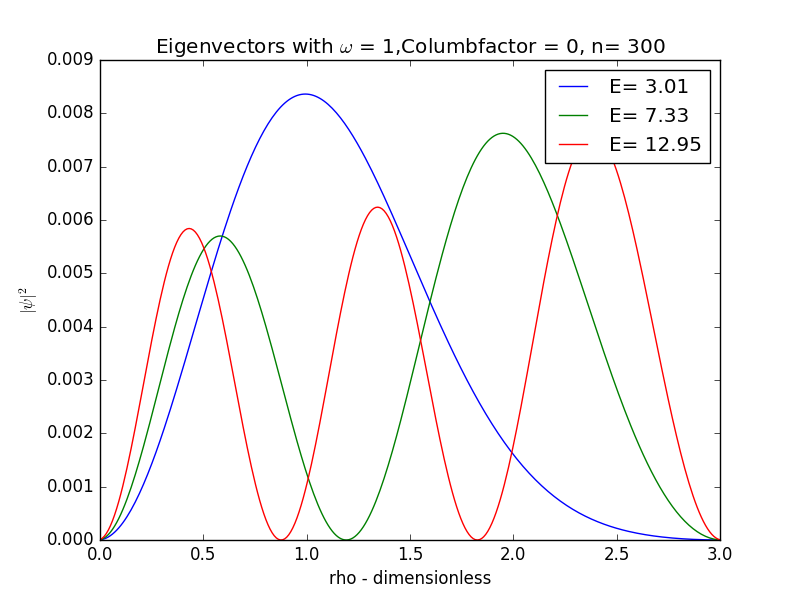
\includegraphics[scale=0.4]{ok_test1_WR=1_CF=0_C=300_rhostop=3}
		\caption{Harmonic oscillator with grid size $=300$, $rho_{max}=3$, $\omega=1$ and Columb Factor $=0$. }
		\label{fig:test1}
	\end{subfigure}
	\begin{subfigure}[b]{0.4\textwidth}
		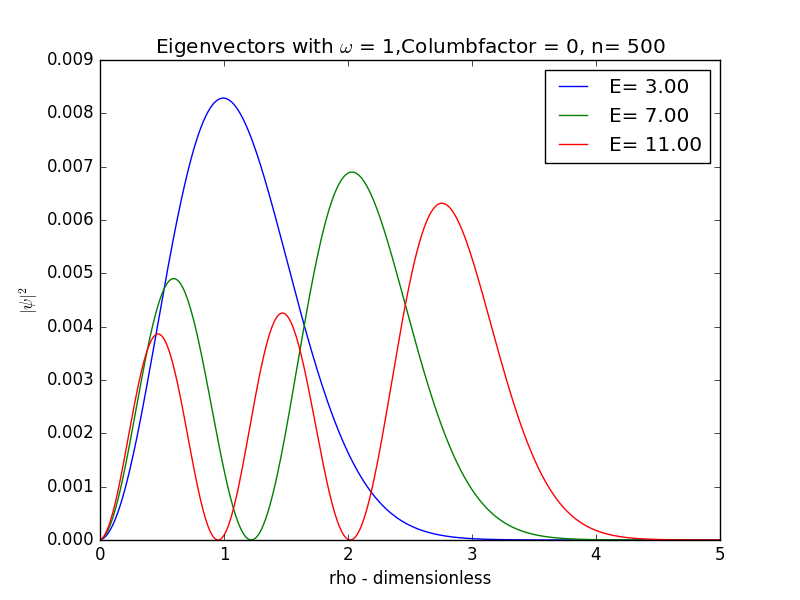
\includegraphics[scale=0.4]{ok_Project_2_Wr=1_Columb_factor=0_n=500_rho_stop=5}
		\caption{Harmonic oscillator with grid size $=500$, $rho_{max}=5$, $\omega=1$ and Columb Factor $=0$. }
		\label{fig:goodtest1}
	\end{subfigure}
\end{figure}


%Varying OMEGA in case 1
In the general case with no interaction term ($C_F = 0$) we want to see how the strength of the oscillator affects the distribution. We used the recommended values of $\omega = (0.01, 0.5, 1, 5)$. In figure \ref{fig:varyingomega} we notice that for a high omega the distribution is pushed towards lower $\rho$ values as the potential gets very steep and the electrons are forces towards the center of the well. The eigenvalues for the energy for the three lowest states seen in table \ref{tab:varying_omega} all increase as the potential increases.

\begin{table}
	\caption{Energy for the 3 lowest eigenvalues for 4 different potential coefficients}
	\begin{center}
		\begin{tabular}{|c||c|c|c|}
			\hline
			Eigenvalue & $\lambda_1$ & $\lambda_2$ & $\lambda_3$ \\
			\hline
			\hline
			$\omega=0.01$ & 0.599 & 0.968 & 1.347  \\
			\hline
			$\omega=0.5$ & 3.001 & 5.710 & 8.464 \\
			\hline
			$\omega=1$ & 4.058 & 7.910 & 11.82 \\
			\hline
			$\omega=5$ & 8.323 & 17.03 & 25.85 \\
			\hline
		\end{tabular}
	\end{center}
	\label{tab:varying_omega}
\end{table}%


%%WITH interaction term case 2
We then focus on the part where we let the interaction term is 1, and want to see how this affects the ground state of the oscillator. To make the results more comparable we use the same range of $\omega = (0.01, 0.5, 1, 5)$ as the previous part. In figure \ref{fig:varyingomegainteracting} one sees that while including the interaction term the wave-function gets pushed outwards from the center of mass. Other that this it is important to note that the eigenvalues are substantially higher in this case. 


\begin{figure}
	\centering
	\begin{subfigure}[b]{0.4\textwidth}
		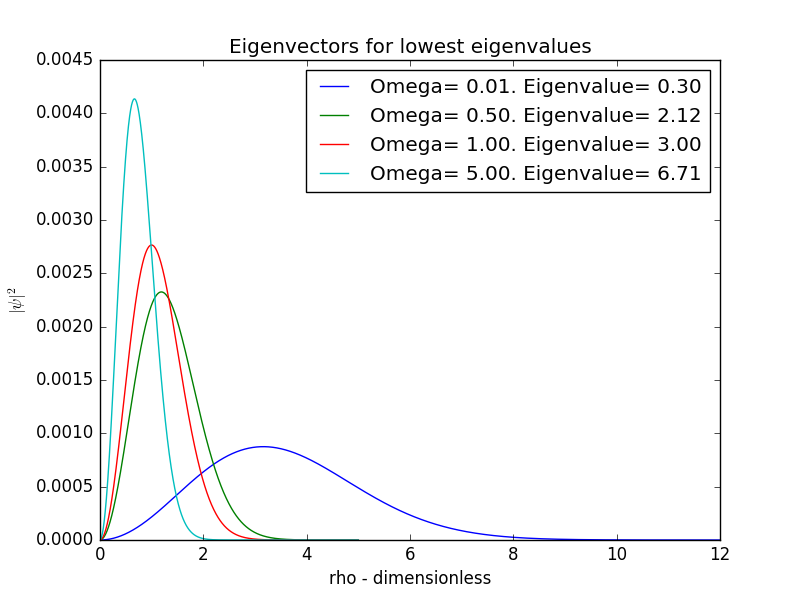
\includegraphics[scale=0.4]{ok_Project_2_Wr=varying_omega}
		\caption{Eigenstates for the lowest energies with varying harmonic oscillator potential strength $C_F = 0$}
		\label{fig:varyingomega}
	\end{subfigure}
	\begin{subfigure}[b]{0.4\textwidth}
		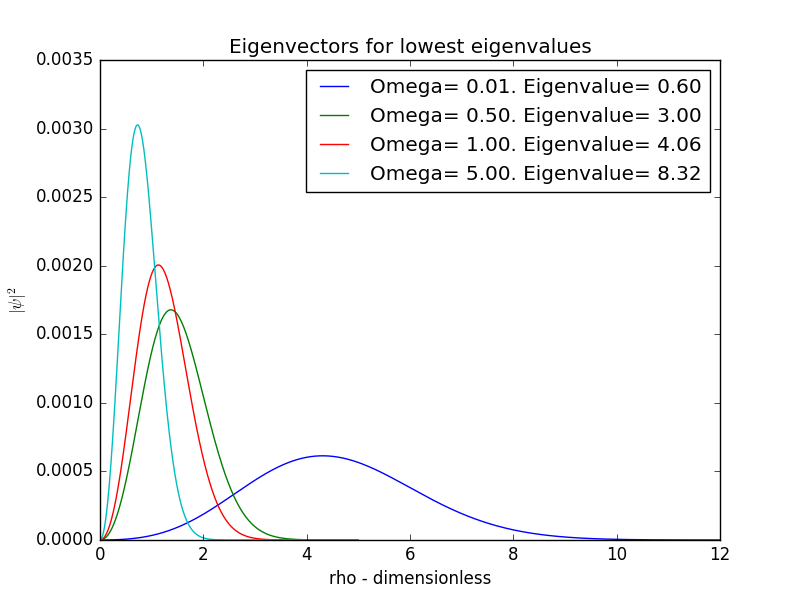
\includegraphics[scale=0.4]{ok_Project_2_Wr=_interaction_varying_omega}
		\caption{Eigenstates for the lowest energies with varying harmonic oscillator potential strength in the interacting case with the $C_F = 1$}
		\label{fig:varyingomegainteracting}
	\end{subfigure}
	
\end{figure}


\subsection{Scaling and flops}
To check the performance and scaling with respect to the grid size, an brute force test that runs the algorithm for different n from 50 to 1000 was performed. Then to find the scaling one approximates the total number of flops with time spend expresses this as a relation which is expected to become more precise for large n
\begin{align}
T \propto n^{a} 
\end{align}
\begin{align}
log_{10}(T) \approx a\cdot log_{10}(n)
\label{eq:scaling}
\end{align}
In figure \ref{fig:scaling} one sees that there is a relation between the grid size and the number of operations. After doing a linear regression on the data with equation \ref{eq:scaling} one finds that 
\begin{align}
T \approx n^{4.0}
\end{align}
This means that the Jacobi's method scales poorly with increasing grid size. Note that these values are expected to be hardware dependent as the number of operations per second varies with the computer, but the values are nevertheless guiding in evaluating the algorithm. The built in method of divide-and-conquer scales much better and is already faster at $n=50$. The memory requirements for both methods would also be interesting to study how Jacobi's method does with respect to this dimension as well. From the results of this scaling test we used the armadillo method for $n>200$ to increase the speed of our calculations as the Jacobi's method simply was to slow in this regime (1 hour for 1000x1000 compared to 0.7 s is a no-brainer). 
\begin{figure}
	\centering
	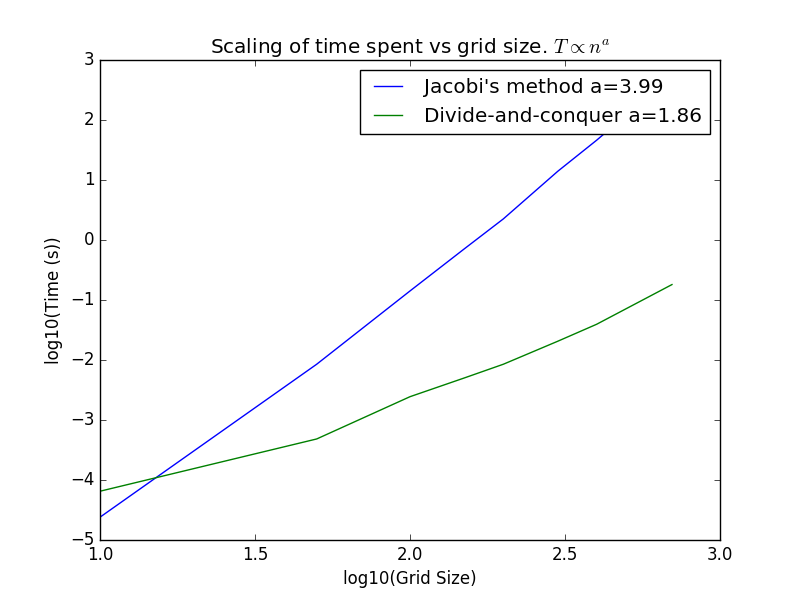
\includegraphics[scale=0.5]{Project2_scaling_time}
	\caption{Time spend on finding eigenvalues/vectors for Jacobi's method and the Divide-and-conquer method.  This data is from a run on a Macbook Pro 13' }
	\label{fig:scaling}
\end{figure}




\section*{Conclusion}
Jacobi's method is an easy to implement method for finding eigenvalues and eigenvectors for linear algebra problems with symmetric, square matrices up to 1000x1000. Since the scaling behavior is poor ($time \approx n^{4}$) for tridiagonal problems, is it not useful as an algorithm for matrices larger that this size. 
For the numerical experiments with the electrons we see that with these methods get the same dimensionless energy eigenvalues(3,7,11) for the c.o.m part as analytical methods achieve for the non-interacting case, and we can in theory handle arbitrary radial potentials as we could change the input in the program. As expected, increasing the potential strength $\omega$ will keep the particles closer to the center-of-mass and lowering it will give the particles more freedom as they are less confined.  When including the interaction term of the type $1/r$ we see that the states are pushed even further out for an arbitrary $\omega$. 


		
\begin{thebibliography}{3}
			
	\bibitem{M.Hjort-Jensen_CompFys}
	Morten Hjort-Jensen
	\emph{ Computational Physics Lecture Notes Fall 2015}
	Department of Physics, University of Oslo
	2015
	\url{https://github.com/CompPhysics/ComputationalPhysics/blob/master/doc/Lectures/lectures2015.pdf}
	
	\bibitem{Divide-and-conquer}
	Wikipedia: Divide-and-conquer method
	\url{https://en.wikipedia.org/wiki/Divide-and-conquer_eigenvalue_algorithm}
	
	
	\bibitem{Armadillo}
	Armadillo package for c++
	\url{http://arma.sourceforge.net/}
	
	
	\bibitem{Project1}
	Ask J. Markestad, Thorbjørn V. Larsen
	\emph{  Project 1: Vector and Matrix Operations in c++}
	\url{https://github.com/ajmarkestad/Fys4150/blob/master/Project1/Project1.pdf}
	
	\bibitem{two_electorn_analysis}
	M. Taut
	\emph{ Two electrons in an external oscillator potential: Particular analytic solutions of a Coulomb correlation problem}
	Phys. Rev. A 48, 3561 – Published 1 November 1993
	\url{http://journals.aps.org/pra/abstract/10.1103/PhysRevA.48.3561}			
			
			
			
\end{thebibliography}
		
		
		
		
		
		
		
		
		
%__________________________________________________________________________
\end{document}